\section{Vererbung (Inheritance)}
	Vererbung ist ein Konzept, das es erlaubt, neue Klassen auf Basis von alten Klassen zu definieren. Die neuen (Unter-, Sub-) Klassen besitzen, ohne Eingriffe in den
	Sourcecode der bereits bestehenden (Ober-, Basis-, Super-) Klassen, all deren Eigenschaften, sie $erben$ deren Verhalten und Daten. Den Vorgang der Vererbung nennt man $Ableiten$.\linebreak
	\begin{minipage}[t]{6.5 cm}
		\subsection{Einsatz der Vererbung \verweiscpp{13.1}}
		\begin{compactitem}
			\item Bestehende Klassen erweitern (zus�tzliche Attribute und Elementfunktionen)
			\item Bestehende Methoden einer Basisklasse �ndern (�berschreiben)
			\item Einsatz nur wenn eine \textbf{IST-EIN ("is a")} Beziehung besteht (z.B. Baum \textbf{ist eine} Pflanze, Blume \textbf{ist eine} Pflanze)
			\linebreak
		\end{compactitem}
		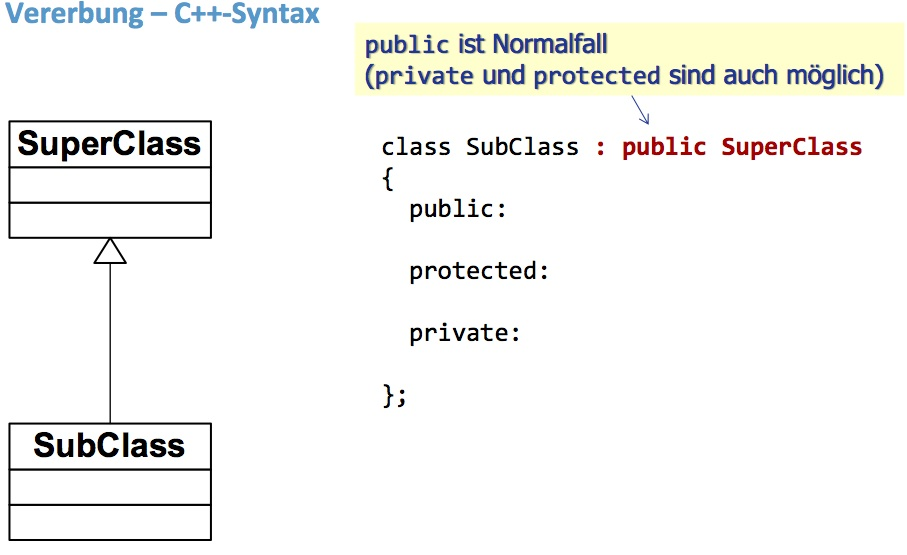
\includegraphics[width=1\textwidth]{pics/bsp_Vererbung.jpg}
		\subsection{Ableiten einer Klasse \verweiscpp{13.2}}
			Der Syntax der Ableitung einer Klasse ist oben aufgef�hrt. Als weiteres Beispiel ist im Anhang das Beispiel des ComicCharacters und SuperHero eingef�gt. SuperHero \textbf{ist ein} ComicCharacter.
			\begin{compactitem}
				\item friend-Beziehungen werden nicht vererbt
				\item Ein Objekt einer Oberklasse kann Objekte einer beliebigen Unterklasse aufnehmen
				\item Ein Objekt einer Unterklasse kann keine Objekte der Oberklasse aufnehmen
				\item Ein Objekt einer vererbten Klasse enth�lt alle Teile der Basisklasse und zus�tzlich noch die spezifischen eigenen Teile.
				\item Das Objekt ist somit mindestens so gross wie jenes der Basisklasse (es gibt keine Vererbung $by$ $reference$)
				\linebreak
			\end{compactitem}
				
	\end{minipage}	
	\hspace*{0.5cm}
	\begin{minipage}[t]{12 cm}
	\subsection{Zugriff auf Elemente der Basisklasse \verweiscpp{13.6}}
		\textbf{Bei Vererbung mit public (Normalfall):}
			\begin{compactitem}
				\item Zugriff m�glich auf alle public- und protected- Elemente der Basisklasse, die Zugriffsrechte 
				(public, protected) der Basisklasse werden in der abgeleiteten Klasse beibehalten
				\item kein Zugriff auf private-Elemente der Basisklasse
				\linebreak
			\end{compactitem}
		\textbf{Bei Vererbung mit protected:}
			\begin{compactitem}
				\item Zugriff m�glich auf alle public- und protected- Elemente der Basisklasse, die Zugriffsrechte 
				von public und protected der Basisklasse werden in der abgeleiteten Klasse zu protected
				\item kein Zugriff auf private-Elemente der Basisklasse
				\linebreak
			\end{compactitem}
		\textbf{Bei Vererbung mit private:}
			\begin{compactitem}
				\item Zugriff m�glich auf alle public- und protected- Elemente der Basisklasse, die Zugriffsrechte 
				von public und protected der Basisklasse werden in der abgeleiteten Klasse zu private
				\item kein Zugriff auf private-Elemente der Basisklasse
				\linebreak
			\end{compactitem}
	\subsection{Slicing Problem \verweiscpp{13.3}}
		Links: Beim Kopieren werden nur die ComicCharacter-Teile ber�cksichtigt. Durch das Kopieren wird alles �berfl�ssige weggeschnitten, �brig bleibt ein reines ComicCharacter Objekt im Fall von s f�hrt dies dazu, dass die erweiterten SuperHero Daten und Funktionen verloren gehen.\newline
		Rechts: Hier wird dank des Referenzparameters der gesamte Superheld ausgegeben.\newline
		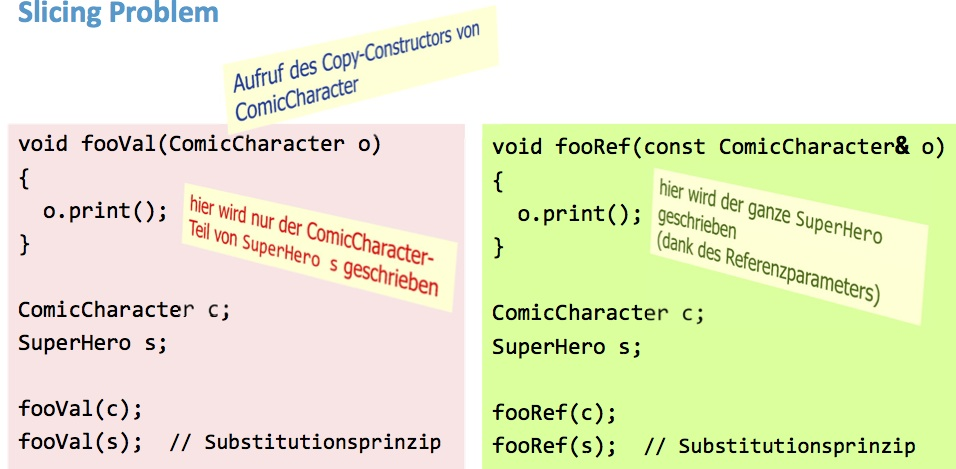
\includegraphics[width=1\textwidth]{pics/SlicingProblem.jpg}
	\end{minipage}	
	